\documentclass[11,]{article}
\usepackage{lmodern}
\usepackage{amssymb,amsmath}
\usepackage{ifxetex,ifluatex}
\usepackage{fixltx2e} % provides \textsubscript
\ifnum 0\ifxetex 1\fi\ifluatex 1\fi=0 % if pdftex
  \usepackage[T1]{fontenc}
  \usepackage[utf8]{inputenc}
\else % if luatex or xelatex
  \ifxetex
    \usepackage{mathspec}
  \else
    \usepackage{fontspec}
  \fi
  \defaultfontfeatures{Ligatures=TeX,Scale=MatchLowercase}
\fi
% use upquote if available, for straight quotes in verbatim environments
\IfFileExists{upquote.sty}{\usepackage{upquote}}{}
% use microtype if available
\IfFileExists{microtype.sty}{%
\usepackage{microtype}
\UseMicrotypeSet[protrusion]{basicmath} % disable protrusion for tt fonts
}{}
\usepackage[margin=1in]{geometry}
\usepackage{hyperref}
\hypersetup{unicode=true,
            pdftitle={The Effect of Economic Events on Votes for the President},
            pdfauthor={Scott Cohn and Samuel Hostetter},
            pdfborder={0 0 0},
            breaklinks=true}
\urlstyle{same}  % don't use monospace font for urls
\usepackage{graphicx,grffile}
\makeatletter
\def\maxwidth{\ifdim\Gin@nat@width>\linewidth\linewidth\else\Gin@nat@width\fi}
\def\maxheight{\ifdim\Gin@nat@height>\textheight\textheight\else\Gin@nat@height\fi}
\makeatother
% Scale images if necessary, so that they will not overflow the page
% margins by default, and it is still possible to overwrite the defaults
% using explicit options in \includegraphics[width, height, ...]{}
\setkeys{Gin}{width=\maxwidth,height=\maxheight,keepaspectratio}
\IfFileExists{parskip.sty}{%
\usepackage{parskip}
}{% else
\setlength{\parindent}{0pt}
\setlength{\parskip}{6pt plus 2pt minus 1pt}
}
\setlength{\emergencystretch}{3em}  % prevent overfull lines
\providecommand{\tightlist}{%
  \setlength{\itemsep}{0pt}\setlength{\parskip}{0pt}}
\setcounter{secnumdepth}{5}
% Redefines (sub)paragraphs to behave more like sections
\ifx\paragraph\undefined\else
\let\oldparagraph\paragraph
\renewcommand{\paragraph}[1]{\oldparagraph{#1}\mbox{}}
\fi
\ifx\subparagraph\undefined\else
\let\oldsubparagraph\subparagraph
\renewcommand{\subparagraph}[1]{\oldsubparagraph{#1}\mbox{}}
\fi

%%% Use protect on footnotes to avoid problems with footnotes in titles
\let\rmarkdownfootnote\footnote%
\def\footnote{\protect\rmarkdownfootnote}

%%% Change title format to be more compact
\usepackage{titling}

% Create subtitle command for use in maketitle
\newcommand{\subtitle}[1]{
  \posttitle{
    \begin{center}\large#1\end{center}
    }
}

\setlength{\droptitle}{-2em}
  \title{The Effect of Economic Events on Votes for the President}
  \pretitle{\vspace{\droptitle}\centering\huge}
  \posttitle{\par}
\subtitle{Resource Economics 312}
  \author{Scott Cohn and Samuel Hostetter}
  \preauthor{\centering\large\emph}
  \postauthor{\par}
  \predate{\centering\large\emph}
  \postdate{\par}
  \date{May 04, 2018}

\usepackage{booktabs}
\usepackage{longtable}
\usepackage{array}
\usepackage{multirow}
\usepackage[table]{xcolor}
\usepackage{wrapfig}
\usepackage{float}
\usepackage{colortbl}
\usepackage{pdflscape}
\usepackage{tabu}
\usepackage{threeparttable}
\usepackage{threeparttablex}
\usepackage[normalem]{ulem}
\usepackage{makecell}

\usepackage{booktabs}
\usepackage{xcolor}
\usepackage{hyperref}
\hypersetup{}
\usepackage{longtable}
\usepackage{array}
\usepackage{multirow}
\usepackage[table]{xcolor}
\usepackage{wrapfig}
\usepackage{float}
\usepackage{colortbl}
\usepackage{pdflscape}
\usepackage{tabu}
\usepackage{threeparttable}
\usepackage{threeparttablex}
\usepackage[normalem]{ulem}
\usepackage{makecell}
\usepackage{dcolumn}

\begin{document}
\maketitle
\begin{abstract}
The Presidential Equation is a logistic probability model created by
Yale University Professor Ray C. Fair to estimate the Democratic share
of the two party votes in any given U.S. presidential election. Fair
incorporates both economic and political variables to predict which
party will gain the majority of votes. This paper recreates and analyzes
the significance of Fair's popular election model. We then provided a
forecast for the 2020 presidential election. We found Fair's model to
hold strong prediction power, providing accurate foresight for every
election from 1916 to today. However, the significance of some variables
used in his predictions is quite low, leading to questions on how the
model remains accurate.
\end{abstract}

\providecommand{\tightlist}{%
  \setlength{\itemsep}{0pt}\setlength{\parskip}{0pt}}

\hypertarget{introduction}{%
\section{Introduction}\label{introduction}}

The ``Presidential Equation'' is a logistic probability model created by
Yale University Professor Ray C. Fair to explain the Democratic share of
votes in any given U.S. presidential election. Fair's model takes into
account economic and social deterministic factors that influence voters'
decisions. This paper will recreate Fair's equation and use it to
develop a forecast for the 2020 presidential election given variable
economic conditions. This paper will also briefly compare the Fair model
to other presidential forecasting models.

\hypertarget{literature-review}{%
\section{Literature Review}\label{literature-review}}

The Fair (\protect\hyperlink{ref-fair_effect_1978}{1978}) paper was
originally published to create a model broad enough where the prominent
voting theories of the time could be tested, and to allow testing of
these theories against each other. The three main theorists Fair cites
in his 1978 paper are Anthony Downs (1957), Gerald H. Kramer (1971), and
George J. Stigler (1973).

\hypertarget{anthony-downs}{%
\subsection{Anthony Downs}\label{anthony-downs}}

Anthony Downs (1957) establishes a disconnect between voter desires and
government desires. In a perfectly informed democracy, every voter
should vote for a government that will maximize social welfare, and the
government that gets elected should do just that. Realistically, Downs
argues, voters and political representatives do not have complete
information, resulting in voting patterns that maximize private economic
welfare and a government whose goal is to attain ``the income, power,
and prestige that come with office'' (Downs
\protect\hyperlink{ref-downs_economic}{1957}). Fair's proposed
relationship between private economic welfare and voting probability was
based on the axioms brought forth by Downs.

\hypertarget{gerald-h.-kramer}{%
\subsection{Gerald H. Kramer}\label{gerald-h.-kramer}}

Gerald Kramer (1971), when he began studying econometrics, was
interested the question of how voting behavior was influenced by
macroeconomic events. Primarily, he focused on votes for the House of
Representatives and Congress. Kramer found that most of the variance in
his predictive model was dependent on the change of personal income in
the short term. Other variables such as coattails, unemployment, and
inflation did not have significant effects. George Stigler (1973) found
an error in Kramer's data, and when the experiment was rerun the output
showed that inflation has a ``modest independent affect'' (Rosenthal
\protect\hyperlink{ref-rosenthal_gerald_2006}{2006}). This effect is
looked at in Fair's modified equation. Kramer also argued in his 1971
paper that the effect of presidential elections is much more influenced
by non-economic events (i.e.~candidate personality) than the elections
of the House and Congress.

\hypertarget{george-j.-stigler}{%
\subsection{George J. Stigler}\label{george-j.-stigler}}

George J. Stigler (1973) reviews Kramer's proposed election model and
disassembles the significance of Kramer's proposed relationships.
Stigler believes voters think about many confounding factors when they
vote, not only Kramer's per-capita income belief. He argues that Kramer
doesn't account for past experiences of the voter and incorrectly
weights recent economic conditions the same as distant conditions
(Stigler \protect\hyperlink{ref-stigler_general_1973}{1973}). Every
voter has a different economic past, so grouping all voters together
into an average per capita income statistic can lead to erroneous
prediction.

At the time of the original paper, the prevailing theory suggested that
a voter looked at the current status and previous performance of the
parties seeking power and voted for the party that maximized ``future
utility'' (Kramer 1971, Stigler 1973). A primary assumption, under this
theory, was that voters are ``self-interested and well-informed'' (Fair
\protect\hyperlink{ref-fair_effect_1978}{1978}). More so, Kramer (1971)
suggests the voter votes for the party if their performance is deemed
``satisfactory''.

\begin{quote}
The standard assumption in {[}election forecasts{]} is that voters hold
the party that controls the presidency accountable for economic events,
rather than, say, the party that controls the Congress (if it is
different) or the Board of Governors of the Federal Reserve System (Fair
\protect\hyperlink{ref-fair_effect_1978}{1978}).
\end{quote}

Therefore, as theory would suggest, economic events greatly influence
the vote for the president in the United States.

\hypertarget{data-and-methods}{%
\section{Data and Methods}\label{data-and-methods}}

\hypertarget{data}{%
\subsection{Data}\label{data}}

The data are provided by Fair via his website. We gathered values dating
from 1916 to 2012, with observations occuring every four years. The data
are limited to a 25 complete observations. With such a small dataset,
degrees of freedom and potential modeling power is less than ideal. Upon
reciept, the data has been cleaned and tidied. There are no missing
values for any of the instances recorded. The data are sourced from the
U.S. Bureau of Economic Analysis (BEA) website. Population data are
taken from the U.S. Department of Commerce (DOC). Ray Fair has compiled
much of the available data to eliminate extraneous variables. The data
are readily available on his personal website alongside links to
previous updates of the model.

\rowcolors{2}{gray!6}{white}
\begin{table}[!h]

\caption{\label{tab:Fair Data}Ray Fair Data}
\centering
\begin{tabular}[t]{rrrrrrrrr}
\hiderowcolors
\toprule
Year & actualVP & I & DPER & DUR & WAR & G & P & Z\\
\midrule
\showrowcolors
1916 & 0.51 & 1 & 1 & 0.00 & 0 & 2.23 & 4.25 & 3\\
1920 & 0.40 & 1 & 0 & 1.00 & 1 & -11.46 & 0.00 & 0\\
1924 & 0.43 & -1 & -1 & 0.00 & 0 & -3.87 & 5.16 & 10\\
1928 & 0.43 & -1 & 0 & -1.00 & 0 & 4.62 & 0.18 & 7\\
1932 & 0.62 & -1 & -1 & -1.25 & 0 & -14.35 & 6.93 & 4\\
\addlinespace
1936 & 0.64 & 1 & 1 & 0.00 & 0 & 11.68 & 2.50 & 9\\
1940 & 0.55 & 1 & 1 & 1.00 & 0 & 3.91 & 0.05 & 8\\
1944 & 0.53 & 1 & 1 & 1.25 & 1 & 4.12 & 0.00 & 0\\
1948 & 0.50 & 1 & 1 & 1.50 & 1 & 3.21 & 0.00 & 0\\
1952 & 0.44 & 1 & 0 & 1.75 & 0 & 1.00 & 2.35 & 7\\
\addlinespace
1956 & 0.42 & -1 & -1 & 0.00 & 0 & -1.25 & 1.91 & 5\\
1960 & 0.50 & -1 & 0 & -1.00 & 0 & 0.67 & 1.98 & 5\\
1964 & 0.61 & 1 & 1 & 0.00 & 0 & 5.03 & 1.24 & 9\\
1968 & 0.42 & 1 & 0 & 1.00 & 0 & 5.04 & 3.09 & 7\\
1972 & 0.37 & -1 & -1 & 0.00 & 0 & 5.83 & 4.81 & 4\\
\addlinespace
1976 & 0.50 & -1 & 0 & -1.00 & 0 & 3.82 & 7.46 & 5\\
1980 & 0.41 & 1 & 1 & 0.00 & 0 & -3.58 & 7.80 & 5\\
1984 & 0.41 & -1 & -1 & 0.00 & 0 & 5.55 & 5.21 & 8\\
1988 & 0.46 & -1 & 0 & -1.00 & 0 & 2.40 & 2.87 & 5\\
1992 & 0.43 & -1 & -1 & -1.25 & 0 & 3.04 & 3.19 & 3\\
\addlinespace
1996 & 0.49 & 1 & 1 & 0.00 & 0 & 3.31 & 2.03 & 4\\
2000 & 0.48 & 1 & 0 & 1.00 & 0 & 2.03 & 1.68 & 7\\
2004 & 0.48 & -1 & -1 & 0.00 & 0 & 2.09 & 2.14 & 2\\
2008 & 0.53 & -1 & 0 & -1.00 & 0 & -1.79 & 2.75 & 2\\
2012 & 0.51 & 1 & 1 & 0.00 & 0 & 1.42 & 1.47 & 1\\
\bottomrule
\end{tabular}
\end{table}
\rowcolors{2}{white}{white}

\hypertarget{the-fair-model}{%
\subsection{The Fair Model}\label{the-fair-model}}

The data are presented in Table 1. The updated Fair equation per 1992 is
as follows:

\[ V_t = \alpha_1 + \alpha_2 G_t\times I_t + \alpha_3 P_t\times I_t + \alpha_4 Z_t\times I_t + \alpha_5 {DPER_t} + \alpha_6 {DUR_t} +\alpha_7 I_t + \alpha_8 {WAR_t} + \mu_t \]

Where, \(\alpha_n\) remain unknown coefficients to be estimated. \(I\)
denotes incumbancy. \(I\) equals 1 if the current president is
Democratic, -1 if Republican, 0 otherwise.\footnote{\(I\) serves two
  functions in Fair's model. First, it interacts with each respective
  coeffiecent to flip the sign of economic variables to either increase
  the chance of Republicans to win (decreasing \(V_t\)) or increase the
  chance of Democrats to win (increasing \(V_t\)). Additionally, \(I\)
  holds a coefficient of its own to demonstrate the effect incumbancy
  has on voters' decisions.} A secondary model testing \(I\) as a binay
variable is included in the discussion section of this paper. \(G\) has
been modified to represent the real growth rate of GDP per capita for
the last three quarters of the election year. In contrast to \(G\), a
``short horizon'' variable, \(P\) and \(Z\) are longer term variables
representing the whole term of the administration. \(P\) represents the
absolute value of the growth rate of the GDP deflator for the first
fifteen quarters of the current administration. \(Z\), the ``good news
variable'', is the number of quarters out of the first fifteen of the
current administration where the growth rate of real GDP is greater than
3.2 percent. Fair notes in his construction of the model that
psychological research dictates that people will remember extreme events
more intensely than normal ones; \(Z\) tries to capture the ``extreme
positive growth outcomes'' in accordance with this theory. \(DPER\)
represents the effect of the current president running while they are in
office. \(DPER\) equals 1 if current president that will run is
Democratic, -1 if Republican, and 0 if the current president will not
run while in office. \(DUR\) is the duration of the party in office (0
if the current ruling party has been in the White House for one term;
\(1\times I\) if current party has held office for two terms;
\((1+k) \times I\) for three terms; \((1+2k)\times I\) for four terms;
and so on, where k is a chosen value of 0.25). \(WAR\) is 1 for the
election years during and immediately following a U.S. war (1920, 1944
and 1948) and 0 otherwise.

In forecasts calculated prior to 1996, the original GDP data are
presented in a Laspeyres index, which tended to overstate the effect of
inflation. Following 1996, GDP is calculated using chain-linked volume
series. According to Fair, this more accurately represents the effects
of production on the vote-share by providing a better index for growth
measurement (Fair \protect\hyperlink{ref-fair_effect_1996}{1996}).

The model above is the most recent iteration of Fair's presidential
equation. Table 2 lists the coefficients derived from the data given in
this paper. Table 3 below demostrates the prediction power of Fair's
model. Appendix A shows the full regression table for all regressions
run with different variable combinations. Appendix B shows a graphical
analysis of the predicted outcomes using Fair's model versus the actual
results.

\rowcolors{2}{gray!6}{white}
\begin{table}[!h]

\caption{\label{tab:Fair Coeff}Ray Fair 1992 Model Coefficients}
\centering
\begin{tabular}[t]{lrrrr}
\hiderowcolors
\toprule
term & estimate & std.error & statistic & p.value\\
\midrule
\showrowcolors
(Intercept) & 0.462 & 0.007 & 69.982 & 0.000\\
I & -0.023 & 0.024 & -0.938 & 0.362\\
DPER & 0.045 & 0.015 & 2.927 & 0.009\\
DUR & -0.027 & 0.013 & -2.033 & 0.058\\
WAR & 0.050 & 0.028 & 1.793 & 0.091\\
\addlinespace
I:G & 0.007 & 0.001 & 5.786 & 0.000\\
I:P & -0.009 & 0.003 & -2.834 & 0.011\\
I:Z & 0.008 & 0.003 & 3.153 & 0.006\\
\bottomrule
\end{tabular}
\end{table}
\rowcolors{2}{white}{white}

\rowcolors{2}{gray!6}{white}
\begin{table}[!h]

\caption{\label{tab:Fair VS Actual}Fair Prediction Compared with Actual Democratic Share of Votes}
\centering
\begin{tabular}[t]{rrrr}
\hiderowcolors
\toprule
Year & Fair\_Prediction & Actual\_Vote\_Share & Error\\
\midrule
\showrowcolors
1916 & 51.682 & 50.7 & 0.982\\
1920 & 36.148 & 39.6 & 3.452\\
1924 & 41.737 & 42.8 & 1.063\\
1928 & 41.244 & 43.4 & 2.156\\
1932 & 59.149 & 61.5 & 2.351\\
\addlinespace
1936 & 62.226 & 64.0 & 1.774\\
1940 & 54.983 & 54.7 & 0.283\\
1944 & 53.778 & 53.4 & 0.378\\
1948 & 52.319 & 49.6 & 2.719\\
1952 & 44.710 & 44.4 & 0.310\\
\addlinespace
1956 & 42.906 & 42.0 & 0.906\\
1960 & 50.087 & 49.7 & 0.387\\
1964 & 61.203 & 61.1 & 0.103\\
1968 & 49.425 & 42.4 & 7.025\\
1972 & 38.209 & 37.2 & 1.009\\
\addlinespace
1976 & 51.049 & 50.0 & 1.049\\
1980 & 44.842 & 41.0 & 3.842\\
1984 & 40.877 & 40.6 & 0.277\\
1988 & 46.168 & 45.7 & 0.468\\
1992 & 53.621 & 43.0 & 10.621\\
\addlinespace
1996 & 54.737 & 49.2 & 5.537\\
2000 & 50.262 & 48.4 & 1.862\\
2004 & 48.767 & 48.3 & 0.467\\
2008 & 53.689 & 52.9 & 0.789\\
2012 & 52.010 & 51.1 & 0.910\\
2016 & 49.000 & 48.2 & 0.800\\
\bottomrule
\end{tabular}
\end{table}
\rowcolors{2}{white}{white}

\hypertarget{model-replication-and-adjustments}{%
\subsection{Model Replication and
Adjustments}\label{model-replication-and-adjustments}}

\hypertarget{multicollinearity}{%
\subsubsection{Multicollinearity}\label{multicollinearity}}

Multicollinearity is a common problem with time series data and
indicates a high degree of correlation between two or more independent
variables. When multicollinearity is present, standard errors inflate
and calculated t-values decrease. With deflated \(t\)-values, the
probability of a Type II error (failing to reject an incorrect
hypothesis) increases. Type II errors remove the possibility for correct
inference to be made about coefficients. One method of detecting
multicollinearity is calculating Variation Inflation Factors (\(VIF\))
using the formula below.

\[VIF_k = \frac{1}{1 - R^2_k}\]

\rowcolors{2}{gray!6}{white}
\begin{table}[!h]

\caption{\label{tab:VIF}Variance Inflation Factors for the Ray Fair Regression Model}
\centering
\begin{tabular}[t]{lr}
\hiderowcolors
\toprule
regressor & VIF\\
\midrule
\showrowcolors
I & 17.787\\
DPER & 4.557\\
DUR & 4.145\\
WAR & 2.481\\
I:G & 1.397\\
\addlinespace
I:P & 4.007\\
I:Z & 6.580\\
\bottomrule
\end{tabular}
\end{table}
\rowcolors{2}{white}{white}

The frequently used heuristic for looking at \emph{Variance Inflation
Factors} suggests that any \emph{VIF} greater than \textbf{10} indicates
a problem. The variable \(I\) has a rather high \emph{VIF}. However,
this can be attributed to it's interaction affects with the other
variables in the model.

\hypertarget{heteroskedasticity}{%
\subsubsection{Heteroskedasticity}\label{heteroskedasticity}}

Heteroskedasticity occurs when residual values are different across
independent variable values. In a homoskedastic model, residuals are of
the same magnitude no matter the value of the independent variable. With
unequal variances, a model displays incorrect standard errors, which
makes inference impossible. To test for heteroskedasticity, we ran a
Breusch-Pagan Test (BP Test) at the \(0.05\) significance level.

\[\chi^2 = n\times R^2 \sim \chi^2_{(N-1)}\]

\rowcolors{2}{gray!6}{white}
\begin{table}[!h]

\caption{\label{tab:unnamed-chunk-1}Breusch-Pagan Test for Heteroskedasticity}
\centering
\begin{tabular}[t]{rrrl}
\hiderowcolors
\toprule
statistic & p.value & parameter & method\\
\midrule
\showrowcolors
5.712 & 0.574 & 7 & studentized Breusch-Pagan test\\
\bottomrule
\end{tabular}
\end{table}
\rowcolors{2}{white}{white}

With a calculated \(p\)-value of \(0.574\) for the chi-squared
statistic, we fail to reject the null hypothesis of homoskedasticity for
the model. The variance is constant throughout all values of our
independent variables.

\hypertarget{autocorrelation}{%
\subsubsection{Autocorrelation}\label{autocorrelation}}

Autocorrelation occurs in a model when the disturbances influence each
other over time. With autocorrelation present, standard errors for each
coefficient are wrong and inference would be incorrect. We utilized the
Durbin-Watson test to check for autocorrelation within our data. We used
the \(d\) statistic as calculated below and testing it against the null
hypothesis \(d=2\) at the \(0.05\) significance level.

\[d = \frac{\sum_{t=2}^{T}(e_t-e_{t-1})^2}{\sum_{t=1}^{T}e^2_t}\]

\rowcolors{2}{gray!6}{white}
\begin{table}[!h]

\caption{\label{tab:DurbinWatson}Durbin-Watson Test for Autocorrelation}
\centering
\begin{tabular}[t]{rrll}
\hiderowcolors
\toprule
statistic & p.value & method & alternative\\
\midrule
\showrowcolors
1.684 & 0.2 & Durbin-Watson test & true autocorrelation is greater than 0\\
\bottomrule
\end{tabular}
\end{table}
\rowcolors{2}{white}{white}

The Durbin-Watson test returns a Durbin-Watson statistic that is not
statistically less than 2. This indicates a lack of positive
autocorrelation. We fail to reject the null hypothesis that true
autocorrelation is greater than 0.

\hypertarget{model-specification-and-interpretation}{%
\subsubsection{Model Specification and
Interpretation}\label{model-specification-and-interpretation}}

A full regression table with all coefficients (Table 12) is available in
Appendix A. Specification of the model began with taking all of the
available variables and regressing them on the true Democratic share of
the vote.
\[V_t = \alpha_1 + \alpha_2 G_t + \alpha_3 P_t + \alpha_4 Z_t+ \alpha_5 {DPER_t} + \alpha_6 {DUR_t} +\alpha_7 I_t + \alpha_8 {WAR_t} + \mu_t\]

This first model had an \(R^2\) of \(0.348\) and a calculated
\(F\)-statistic of \(1.295\) on 7 and 17 degrees of freedom. The
\(p\)-value for this statistic was \(0.3107\). This did not indicate
model significance at the 5 percent level. The effects of the parameters
were minimal, and the only parameter that appeared significant was the
intercept (which was significant at the 1 percent level). There seemed
to be too much variablity resulting from various incumbent conditions.

Next, we hypothesized that the party of the incumbent may affect the
economic variables and their contribution to the vote-share. The second
model (designated as ``Interaction'' at the top of Table 12 in Appendix
A) interacted the variable \(I\) with \(G\), \(P\) and \(Z\), while also
leaving non-interacted \(G\), \(P\), and \(Z\) in the model.

\[V_t = \alpha_1 + \alpha_2 G_t\times I_t + \alpha_3 P_t\times I_t + \alpha_4 Z_t\times I_t + \alpha_5 {DPER_t} + \alpha_6 {DUR_t} +\alpha_7 I_t + \alpha_8 {WAR_t} + \alpha_9 G_t + \alpha_{10} P_t + \alpha_{11} Z_t + \mu_t\]
Our adjusted-\(R^2\) in this model jumped to \(0.8155\), with a
calculated \(F\)-statistic of \(11.608\) on 10 and 14 degrees of
freedom. The \(p\)-value for this statistic is significant at less than
the 1 percent level, indicating that the model is highly significant. In
this model, all of the interaction terms are significant at, at least,
the 5 percent level. Other significant parameters include the intercept
and \(DPER\). While removing insignificant variables can introduce
specification bias, we wanted to explore Fair's final model. Fair
removed redundancy in his model by removing the non-interated \(G\),
\(P\), and \(Z\) variables.

Fair's final model is below.

\[V_t = \alpha_1 + \alpha_2 G_t\times I_t + \alpha_3 P_t\times I_t + \alpha_4 Z_t\times I_t + \alpha_5 {DPER_t} + \alpha_6 {DUR_t} +\alpha_7 I_t + \alpha_8 {WAR_t} + \mu_t\]
The model above is the model used from 1992 to present by Ray Fair. This
model has an adjusted-\(R^2\) of \(0.8327\), with a calculated
\(F\)-statistic of \(18.06\). The \(p\)-value for this statistic is
\(1.021e-06\), indicating very high significance. Additionally, all of
the parameters, except \(I\) and \(WAR\) have significance at the 5
percent level (unlike \(WAR\), \(I\) has significant interaction with
other parameters). What happens if we remove the \(WAR\) variable?

\[V_t = \alpha_1 + \alpha_2 G_t\times I_t + \alpha_3 P_t\times I_t + \alpha_4 Z_t\times I_t + \alpha_5 {DPER_t} + \alpha_6 {DUR_t} +\alpha_7 I_t + \mu_t\]
After removing the \(WAR\) variable, the adjusted-\(R^2\) goes down to
\(0.8121\). Many of the parameters become slightly less significant, but
none of them have their coefficients significantly altered. See Table 12
for a side-by-side comparison of the values. We ran a Joint \(F\)-test
to determine whether the \(WAR\) variable is significant.

\rowcolors{2}{gray!6}{white}
\begin{table}[!h]

\caption{\label{tab:unnamed-chunk-2}Joint F-Test for WAR parameter}
\centering
\begin{tabular}[t]{rrrrrr}
\hiderowcolors
\toprule
res.df & rss & df & sumsq & statistic & p.value\\
\midrule
\showrowcolors
17 & 0.014 & NA & NA & NA & NA\\
18 & 0.017 & -1 & -0.003 & 3.214 & 0.091\\
\bottomrule
\end{tabular}
\end{table}
\rowcolors{2}{white}{white}

The results of the Joint \(F\)-test indicate failure to reject the null
hypothesis that the two models are equivalent. Given the higher
adj-\(R^2\) and higher signficance of the individual parameters, our
model will continue to utilize the \(WAR\) variable.

Thus, we return to Fair's model (Table 12, Column 3):
\[V_t = \alpha_1 + \alpha_2 G_t\times I_t + \alpha_3 P_t\times I_t + \alpha_4 Z_t\times I_t + \alpha_5 {DPER_t} + \alpha_6 {DUR_t} +\alpha_7 I_t + \alpha_8 {WAR_t} + \mu_t\]

By looking at the significant coefficients, were able to analyze the
relationship between the independent and dependent variables. First,
both positive economic variables (\(G\) and \(Z\)) positively affected
the party in power. When the economy is doing well, voters tend to
attribute the success to the current president. Interestingly, the
inflation variable, \(P\), negatively affects the party in power. Voters
don't enjoy increasing price levels, which is shown explicitly in the
model. The last significant coefficient is \(DPER\), which indicates if
the current incumbent will run again. Since the coefficient is positive,
voters tend to vote for the incumbent if they decide to run again.

\hypertarget{forecasting}{%
\section{Forecasting}\label{forecasting}}

A key adjunct to this paper is a presidential vote forecast. Fair's
presidential equation is notoriours for it's accuracy in predicting the
outcome of elections. In 2014, Fair constructed a forecast to the 2016
election by setting all non-economic variables to their respective fixed
values and placing predictions on economic variables (Fair 2014). The
three separate forecasts for a booming, continuous, or sluggish economy
provided by Fair indicated a Republican win barring an economic boom.
The economic conditions that followed the 2014 paper resembled his
``Economic Slowdown'' scenario, affirming his preliminary forecast of a
Republican winning the election. Fair's forecast is displayed in Table 7
below.

To further Fair's work, this paper will conduct a forecast for the 2020
presidential election. Our predictions are made similar to the
predictions Fair made during his 2014 forecast. We make the assumption
that his predictions are sound and therefore excluding discussion on
those formulations from this paper. The \(G\), \(P\), \(Z\), \(DPER\),
\(DUR\), and \(I\) variables for the 2020 forecast are as follows:

The non-economic variables in all three scenarios are fixed. \(I\) =
\(-1\) (Republican party is in power), \(DPER\) = \(-1\) (assuming
incumbent president will run again), \(DUR\) = 0 (Republican party has
been in power for only one term), and \(WAR\) = 0. In the ``continued
economic conditions'' scenario, we input the growth rate of per capita
GDP (\(G\)) as the growth rate experienced at the end of 2017 (2017:3 -
2017:4) at the annual rate. The value of 1.85 comes from data taken from
the Federal Reserve Bank of St.~Louis (U.S. Bureau of Economic Analysis
\protect\hyperlink{ref-FRED_1947}{1947}\protect\hyperlink{ref-FRED_1947}{a}).
The absolute value of the GDP deflator (\(P\)) was calculated similarly
to the per capita GDP growth rate, taking economic data from 2017
(2016:4 - 2017:4) and determining the growth rate of inflation at the
annual rate. For the same reason we are excluding discussion of the
derivation of \(G\), we do the same for \(P\). It is explained in depth
in Fair 2014. The calculated value for \(P\) was 2.35 (U.S. Bureau of
Economic Analysis
\protect\hyperlink{ref-us_bureau_of_economic_analysis_gross_1947}{1947}\protect\hyperlink{ref-us_bureau_of_economic_analysis_gross_1947}{b}).
Typically, foreasting with this model occurs using the first 8 quarters
of the current administration, but there have not been 8 quarters yet.
Given there haven't been enough ``good news'' quarters (\(Z\)) yet, the
data are showing an upward trend in GDP per capita growth rate. With
this trend, our estimate of \(Z\) for the ``continued economic
condition'' forecast is 4.

The remaining two scenarios have variable values scaled up or down. For
example, in our ``Large Boom'' scenario, \(G\), or growth rate of GDP
per capita, is nearly doubled to estimate how the growth rate would act
in a booming economy. The three scenarios forecast the Democratic vote
count in 2020 based on three different economic conditions. The next
step is to run the three separate scenarios through Fair's presidential
equation, with the coefficients shown in the first column of Table 2. In
Table 8, the results of the forecast are shown. In all three scenarios,
the Democratic share of votes is under 50 percent, indicating a high
liklihood of a Republican victory in the 2020 election.

\rowcolors{2}{gray!6}{white}
\begin{table}[!h]

\caption{\label{tab:unnamed-chunk-3}2016 Election Forecast}
\centering
\begin{tabular}[t]{lrrrr}
\hiderowcolors
\toprule
Possible Economic Condition & G & P & Z & Forecast\\
\midrule
\showrowcolors
Roughly Continued 2014 Rate & 2.97 & 2.14 & 6 & 0.49\\
Large Boom & 4.00 & 2.14 & 8 & 0.51\\
Economic Slowdown & 1.00 & 1.50 & 2 & 0.44\\
\bottomrule
\end{tabular}
\end{table}
\rowcolors{2}{white}{white}

\rowcolors{2}{gray!6}{white}
\begin{table}[!h]

\caption{\label{tab:unnamed-chunk-3}2020 Election Forecast}
\centering
\begin{tabular}[t]{lrrrr}
\hiderowcolors
\toprule
Possible Economic Condition & G & P & Z & Forecast\\
\midrule
\showrowcolors
Roughly Continued 2017 Rate & 1.62 & 1.36 & 4 & 0.42\\
Large Boom & 3.00 & 2.14 & 8 & 0.39\\
Economic Slowdown & 0.00 & 1.50 & 2 & 0.46\\
\bottomrule
\end{tabular}
\end{table}
\rowcolors{2}{white}{white}

\hypertarget{other-presidential-forecasting-models}{%
\section{Other Presidential Forecasting
Models}\label{other-presidential-forecasting-models}}

Fair's model is praised for it's scope and number of variables. As
election forecasting models have grown in popularity, some of the
emerging models take similiar approaches to Fair. Others, notably
Campbell (\protect\hyperlink{ref-campbell_forecasting_1992}{1992}), opt
for a much tighter model specification with fewer independent variables
to gain similiar accuracy in their estimates.

Other popular general election models (like the polls-plus, polls-only
and now-cast from FiveThirtyEight) combine machine learning algorithms
with regression analysis to make estimations. These models combine poll
results\footnote{``The idea behind an election forecast like
  FiveThirtyEight's is to take polls (`Clinton is ahead by 3 points')
  and transform them into probabilities (`She has a 70 percent chance of
  winning')'' (Silver \protect\hyperlink{ref-silver_users_2016}{2016}).}
with economic data, and run tens of thouseands of simulations once the
models are calibrated to their specifications (Silver
\protect\hyperlink{ref-silver_users_2016}{2016}). Many of these models
are strong in their predictions, but they are less robust at determining
the precise effect of each variable on the outcome. Often, a combination
of machine learning and classical regression techniques in these models
yield the best results.

\hypertarget{discussion}{%
\section{Discussion}\label{discussion}}

The incumbent variable (\(I\)) in Fair's model imposes an equality
constraint. When interpreting the interaction coefficients in front of
\(G\), \(P\), and \(Z\), an assumption is made that the effect of a one
unit change in these variables is identical for when \(I\) equals \(1\)
or \(-1\). Or, a change in economic conditions has the same effect on
voter preference no matter which party is currently in office. The
assumption of equal effects can be naive, for the two parties are known
to have unequal effects on the economy.

To test the validity of the restriction, we ran Fair's model with the
incumbency variable split into two groups: Democrats and Republicans. To
satisfy these conditions, we removed \(I\) and replaced it with binary
variable \(DemI\), which equals \(1\) when a democratic president is in
office and \(0\) when a Republican president is in office. The split
allows for two sets of coefficients to be analyzed: one when a Democrat
is in office and one when a Republican is in office. Below are the
coefficients and Variation Inflation Factors.

\[V_t = \alpha_1 + \alpha_2 G_t DemI_t + \alpha_3 P_t DemI_t + \alpha_4 Z_t  DemI_t + \alpha_5 {DPER_t} + \alpha_6 {DUR_t} +\alpha_7 DemI_t + \alpha_8 {WAR_t} + \alpha_9 G_t + \alpha_{10} P_t + \alpha_{11} Z_t + \mu_t\]

\rowcolors{2}{gray!6}{white}
\begin{table}[!h]

\caption{\label{tab:Dem_Coeff}Split Incumbent Coefficents}
\centering
\begin{tabular}[t]{lrrrr}
\hiderowcolors
\toprule
term & estimate & std.error & statistic & p.value\\
\midrule
\showrowcolors
(Intercept) & 0.494 & 0.033 & 14.863 & 0.000\\
DemI & -0.041 & 0.057 & -0.722 & 0.482\\
DPER & 0.047 & 0.019 & 2.421 & 0.030\\
DUR & -0.028 & 0.016 & -1.714 & 0.109\\
WAR & 0.035 & 0.039 & 0.899 & 0.384\\
\addlinespace
G & -0.008 & 0.002 & -4.402 & 0.001\\
P & 0.006 & 0.005 & 1.301 & 0.214\\
Z & -0.007 & 0.004 & -1.849 & 0.086\\
DemI:G & 0.014 & 0.003 & 5.253 & 0.000\\
DemI:P & -0.019 & 0.007 & -2.816 & 0.014\\
DemI:Z & 0.016 & 0.006 & 2.756 & 0.015\\
\bottomrule
\end{tabular}
\end{table}
\rowcolors{2}{white}{white}

\rowcolors{2}{gray!6}{white}
\begin{table}[!h]

\caption{\label{tab:Dem_Vif}Variance Inflation Factors for Split Incumbent}
\centering
\begin{tabular}[t]{lr}
\hiderowcolors
\toprule
regressor & VIF\\
\midrule
\showrowcolors
DemI & 22.100\\
DPER & 6.458\\
DUR & 5.649\\
WAR & 4.438\\
G & 2.583\\
\addlinespace
P & 2.883\\
Z & 3.780\\
DemI:G & 2.978\\
DemI:P & 4.349\\
DemI:Z & 10.320\\
\bottomrule
\end{tabular}
\end{table}
\rowcolors{2}{white}{white}

The ``Split Incumbent'' model brings party-specific insights on the
effect economic factors have on voter preferences. The adj-\(R^2\) for
Fair's equal effect model is \(0.833\) (Table 12) compared to our split
incumbent model's adj-\(R^2\) value of \(0.815\) (Table 13). The similar
strength of the models show that splitting the incumbent interaction
term does not adversely affect the significance of the model.

Our model brings back the \(G\), \(P\), and \(Z\) independent variables
that Fair removed. In the Split Incumbent model, the coefficients in
front of these non-interacted terms indicate the effect of a one unit
change in the economic condition has on the democratic share of votes
when a Republican is in office. The coefficients are then changed by the
interaction term when a Democratic president is in office.

If Fair's model is correct, we are to expect equal but opposite
coefficients for when Republicans or Democrats are in office. However,
the economic variable \(P\) has significantly different effects on voter
behavior depending on who is in office. When a Republican is in office,
a one percent increase in the absolute value of the growth rate of the
GDP deflator increases the Democratic share of the two-party vote by
\(0.006\) percent. When a Democrat is in office, a one percent increase
in the absolute value of the growth rate of the GDP deflator decreases
the Democratic share by \(0.013\). With such a significant difference of
effects, the Split Incumbent model illuminates the equality constraint
within Fair's model.

\hypertarget{conclusion}{%
\section{Conclusion}\label{conclusion}}

Many traditional journalists conduct revisionist history when talking
about the events leading up to an outcome. Data journalism and election
forecasting reverse the methods of traditional outlets of political
media. Forecasting models circumvent the political hype surrounding
election predictions and instead focus on concrete economic and politcal
data. Often, correctness is praised higher than model confidence.
Regardless of how well specified the model is, an incorrect forecast is
still an incorrect forecast. Traditional media does not care if
specificiation bias leads to more accurate forecasts --- they
exclusively care about who will win the Presidency.

Problems often arise in interpretations of these models. These forecasts
and model predictions are representations of uncertainty. To the
untrained eye, these forecasts can seem more absolute than they are.
Using the example of a presidential election, if the model has a point
estimate of 52 percent of the votes going towards the Republican nominee
there can be a confidence interval that spans a 49 percent outcome to a
55 percent outcome. Both ends of this interval \emph{can be} equally
likely. This paper brings a scrutinizing eye to one of the most accurate
election equations: the Fair model. By testing for common errors in time
series analysis (such as autocorrelation and heteroskedasticity), we
explored possible weaknesses in the model's accuracy. Many of our
attempts came up fruitless. Our Split Incumbent model showed how
interpretation of Fair's coefficients can be skewed. But, the two models
showed nearly identical accuracy. Even when run through our gauntlet of
specification tests, the Fair model remains robust.

The forecast section of this paper provides insight on how the Fair
model can be used to give preliminary estimates for upcoming elections.
A key distinction between the forecast and the model is a decrease in
confidence. The economic equation Fair uses to generate his steadfast
predictions relies on data only available during the current election
year. The forecast in this paper generates three separate estimates for
three of the variables (\(G\),\(P\), and \(Z\)) based on different
possible economic scenarios leading up to the 2020 election. It is very
possible that none of the exact scenarios pan out in the coming years.
In time, the forecast's strength can be tried with actual economic
variables and actual election results. Fair's latest forecast in 2014
correctly forecasted a Republican win in 2016 with respect to actual
economic conditions. Our 2018 forecast run through Fair's model
predictsa Republican win in the 2020 presidential election, no matter
the economic scenario.

\clearpage

\hypertarget{appendix-a-regression-results}{%
\section{Appendix A --- Regression
Results}\label{appendix-a-regression-results}}

\begin{table}[!htbp] \centering 
  \caption{Regression Results} 
  \label{} 
\begin{tabular}{@{\extracolsep{5pt}}lD{.}{.}{-3} D{.}{.}{-3} D{.}{.}{-3} D{.}{.}{-3} } 
\\[-1.8ex]\hline 
\hline \\[-1.8ex] 
\\[-1.8ex] & \multicolumn{4}{c}{actualVP} \\ 
 & \multicolumn{1}{c}{Full} & \multicolumn{1}{c}{Interaction} & \multicolumn{1}{c}{Fair} & \multicolumn{1}{c}{No WAR} \\ 
\\[-1.8ex] & \multicolumn{1}{c}{(1)} & \multicolumn{1}{c}{(2)} & \multicolumn{1}{c}{(3)} & \multicolumn{1}{c}{(4)}\\ 
\hline \\[-1.8ex] 
 I & 0.017 & -0.020 & -0.023 & -0.008 \\ 
  & (0.043) & (0.028) & (0.024) & (0.024) \\ 
  & & & & \\ 
 DPER & 0.037 & 0.047^{**} & 0.045^{***} & 0.051^{***} \\ 
  & (0.042) & (0.019) & (0.015) & (0.016) \\ 
  & & & & \\ 
 DUR & -0.042 & -0.028 & -0.027^{*} & -0.020 \\ 
  & (0.036) & (0.016) & (0.013) & (0.013) \\ 
  & & & & \\ 
 WAR & 0.018 & 0.035 & 0.050^{*} &  \\ 
  & (0.073) & (0.039) & (0.028) &  \\ 
  & & & & \\ 
 G & -0.001 & -0.001 &  &  \\ 
  & (0.003) & (0.002) &  &  \\ 
  & & & & \\ 
 P & -0.005 & -0.004 &  &  \\ 
  & (0.007) & (0.003) &  &  \\ 
  & & & & \\ 
 Z & 0.006 & 0.000 &  &  \\ 
  & (0.006) & (0.003) &  &  \\ 
  & & & & \\ 
 I:G &  & 0.007^{***} & 0.007^{***} & 0.007^{***} \\ 
  &  & (0.001) & (0.001) & (0.001) \\ 
  & & & & \\ 
 I:P &  & -0.010^{**} & -0.009^{**} & -0.011^{***} \\ 
  &  & (0.003) & (0.003) & (0.003) \\ 
  & & & & \\ 
 I:Z &  & 0.008^{**} & 0.008^{***} & 0.006^{**} \\ 
  &  & (0.003) & (0.003) & (0.002) \\ 
  & & & & \\ 
 Constant & 0.467^{***} & 0.473^{***} & 0.462^{***} & 0.466^{***} \\ 
  & (0.045) & (0.021) & (0.007) & (0.007) \\ 
  & & & & \\ 
Observations & \multicolumn{1}{c}{25} & \multicolumn{1}{c}{25} & \multicolumn{1}{c}{25} & \multicolumn{1}{c}{25} \\ 
R$^{2}$ & \multicolumn{1}{c}{0.348} & \multicolumn{1}{c}{0.892} & \multicolumn{1}{c}{0.881} & \multicolumn{1}{c}{0.859} \\ 
Adjusted R$^{2}$ & \multicolumn{1}{c}{0.079} & \multicolumn{1}{c}{0.815} & \multicolumn{1}{c}{0.833} & \multicolumn{1}{c}{0.812} \\ 
Residual Std. Error & \multicolumn{1}{c}{0.067 (df = 17)} & \multicolumn{1}{c}{0.030 (df = 14)} & \multicolumn{1}{c}{0.029 (df = 17)} & \multicolumn{1}{c}{0.030 (df = 18)} \\ 
F Statistic & \multicolumn{1}{c}{1.295 (df = 7; 17)} & \multicolumn{1}{c}{11.608$^{***}$ (df = 10; 14)} & \multicolumn{1}{c}{18.060$^{***}$ (df = 7; 17)} & \multicolumn{1}{c}{18.286$^{***}$ (df = 6; 18)} \\ 
\hline \\[-1.8ex] 
\textit{Notes:} & \multicolumn{4}{l}{$^{***}$Significant at the 1 percent level.} \\ 
 & \multicolumn{4}{l}{$^{**}$Significant at the 5 percent level.} \\ 
 & \multicolumn{4}{l}{$^{*}$Significant at the 10 percent level.} \\ 
\end{tabular} 
\end{table}

\begin{table}[!htbp] \centering 
  \caption{Regression Results} 
  \label{} 
\begin{tabular}{@{\extracolsep{5pt}}lD{.}{.}{-3} } 
\\[-1.8ex]\hline 
\hline \\[-1.8ex] 
\\[-1.8ex] & \multicolumn{1}{c}{actualVP} \\ 
 & \multicolumn{1}{c}{Split Incumbent} \\ 
\hline \\[-1.8ex] 
 DemI & -0.041 \\ 
  & (0.057) \\ 
  & \\ 
 DPER & 0.047^{**} \\ 
  & (0.019) \\ 
  & \\ 
 DUR & -0.028 \\ 
  & (0.016) \\ 
  & \\ 
 WAR & 0.035 \\ 
  & (0.039) \\ 
  & \\ 
 G & -0.008^{***} \\ 
  & (0.002) \\ 
  & \\ 
 P & 0.006 \\ 
  & (0.005) \\ 
  & \\ 
 Z & -0.007^{*} \\ 
  & (0.004) \\ 
  & \\ 
 DemI:G & 0.014^{***} \\ 
  & (0.003) \\ 
  & \\ 
 DemI:P & -0.019^{**} \\ 
  & (0.007) \\ 
  & \\ 
 DemI:Z & 0.016^{**} \\ 
  & (0.006) \\ 
  & \\ 
 Constant & 0.494^{***} \\ 
  & (0.033) \\ 
  & \\ 
Observations & \multicolumn{1}{c}{25} \\ 
R$^{2}$ & \multicolumn{1}{c}{0.892} \\ 
Adjusted R$^{2}$ & \multicolumn{1}{c}{0.815} \\ 
Residual Std. Error & \multicolumn{1}{c}{0.030 (df = 14)} \\ 
F Statistic & \multicolumn{1}{c}{11.608$^{***}$ (df = 10; 14)} \\ 
\hline \\[-1.8ex] 
\textit{Notes:} & \multicolumn{1}{l}{$^{***}$Significant at the 1 percent level.} \\ 
 & \multicolumn{1}{l}{$^{**}$Significant at the 5 percent level.} \\ 
 & \multicolumn{1}{l}{$^{*}$Significant at the 10 percent level.} \\ 
\end{tabular} 
\end{table}

\hypertarget{appendix-b-graph}{%
\section{Appendix B --- Graph}\label{appendix-b-graph}}

\begin{center}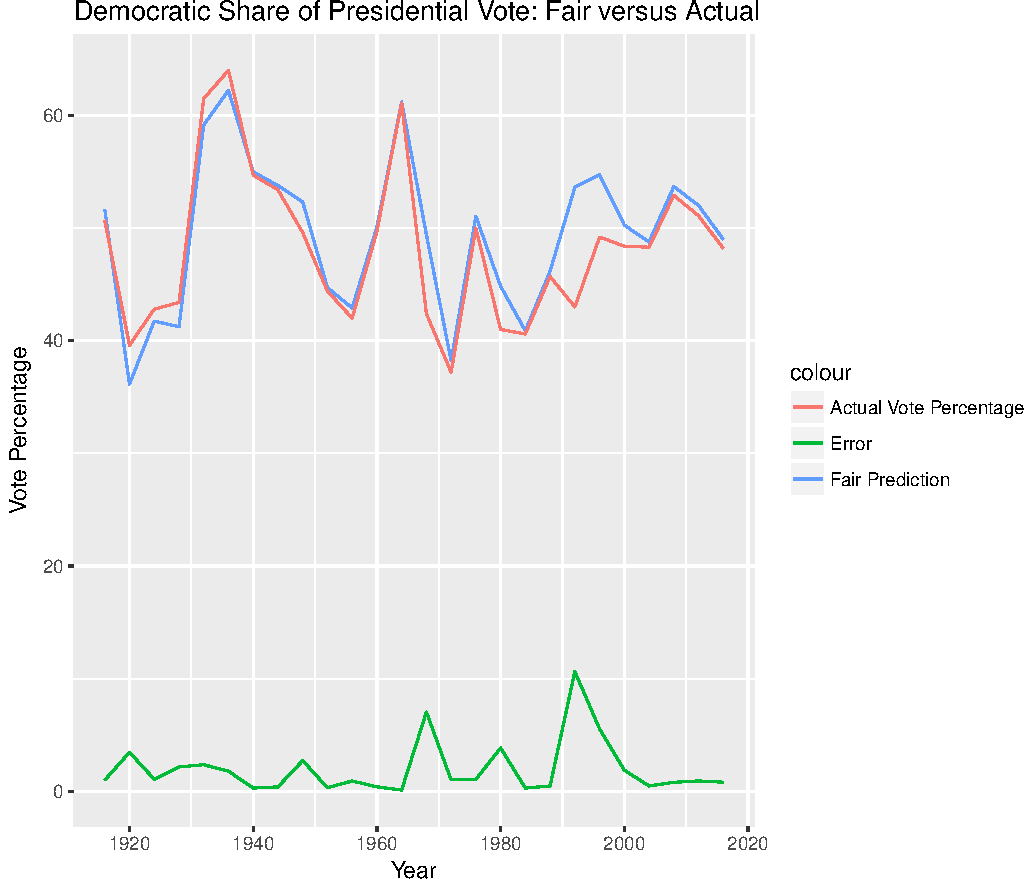
\includegraphics[width=0.65\linewidth]{WriteUp_files/figure-latex/unnamed-chunk-4-1} \end{center}

\hypertarget{technical-documentation}{%
\section{Technical Documentation}\label{technical-documentation}}

Written using R (R Core Team \protect\hyperlink{ref-R}{2013}).

Packages used:

\begin{itemize}
\tightlist
\item
  knitr, Xie (\protect\hyperlink{ref-R-knitr}{2018})
\item
  MASS, Venables and Ripley (\protect\hyperlink{ref-MASS}{2002})
\item
  xtable, Dahl (\protect\hyperlink{ref-xtable}{2016})
\item
  mosaic, Pruim, Kaplan, and Horton
  (\protect\hyperlink{ref-mosaic}{2017})
\item
  readxl, Wickham and Bryan (\protect\hyperlink{ref-readxl}{2017})
\item
  dplyr, Wickham et al. (\protect\hyperlink{ref-dplyr}{2017})
\item
  Stargazer, Hlavac (\protect\hyperlink{ref-stargazer}{2018})
\item
  DataExplorer, Cui (\protect\hyperlink{ref-DataExplorer}{2018})
\item
  tidyverse, Wickham (\protect\hyperlink{ref-tidyverse}{2017})
\item
  randomForest, Liaw and Wiener
  (\protect\hyperlink{ref-randomForest}{2002})
\item
  car, Fox and Weisberg (\protect\hyperlink{ref-car}{2011})
\item
  gplot2, Wickham (\protect\hyperlink{ref-ggplot2}{2009})
\item
  sjPlot, Lüdecke (\protect\hyperlink{ref-sjPlot}{2018})
\item
  broom, Robinson (\protect\hyperlink{ref-broom}{2018})
\item
  texreg, Leifeld (\protect\hyperlink{ref-texreg}{2013})
\item
  forecast, Hyndman and Khandakar
  (\protect\hyperlink{ref-forecast}{2008})
\item
  lmtest, Zeileis and Hothorn (\protect\hyperlink{ref-lmtest}{2002})
\end{itemize}

\hypertarget{references}{%
\section*{References}\label{references}}
\addcontentsline{toc}{section}{References}

\hypertarget{refs}{}
\leavevmode\hypertarget{ref-campbell_forecasting_1992}{}%
Campbell, James E. 1992. ``Forecasting the Presidential Vote in the
States.'' \emph{American Journal of Political Science} 36 (2):386--407.
\url{https://doi.org/10.2307/2111483}.

\leavevmode\hypertarget{ref-DataExplorer}{}%
Cui, Boxuan. 2018. \emph{DataExplorer: Data Explorer}.
\url{https://CRAN.R-project.org/package=DataExplorer}.

\leavevmode\hypertarget{ref-xtable}{}%
Dahl, David B. 2016. \emph{Xtable: Export Tables to Latex or Html}.
\url{https://CRAN.R-project.org/package=xtable}.

\leavevmode\hypertarget{ref-downs_economic}{}%
Downs, Anthony. 1957. ``An Economic Theory of Political Action in a
Democracy.'' \emph{Journal of Political Economy} 65 (2 (Apr.,
1957)):135--50. \url{http://www.jstor.org/stable/1827369}.

\leavevmode\hypertarget{ref-fair_effect_1978}{}%
Fair, Ray C. 1978. ``The Effect of Economic Events on Votes for
President.'' \emph{The Review of Economics and Statistics} 60
(2):159--73. \url{https://doi.org/10.2307/1924969}.

\leavevmode\hypertarget{ref-fair_effect_1996}{}%
---------. 1996. ``The Effect of Economic Events on Votes for President:
1992 Update.'' \emph{Political Behavior} 18 (2):119--39.
\url{http://www.jstor.org/stable/586603}.

\leavevmode\hypertarget{ref-car}{}%
Fox, John, and Sanford Weisberg. 2011. \emph{An R Companion to Applied
Regression}. Second. Thousand Oaks CA: Sage.
\url{http://socserv.socsci.mcmaster.ca/jfox/Books/Companion}.

\leavevmode\hypertarget{ref-stargazer}{}%
Hlavac, Marek. 2018. \emph{Stargazer: Well-Formatted Regression and
Summary Statistics Tables}. Bratislava, Slovakia: Central European
Labour Studies Institute (CELSI).
\url{https://CRAN.R-project.org/package=stargazer}.

\leavevmode\hypertarget{ref-forecast}{}%
Hyndman, Rob J, and Yeasmin Khandakar. 2008. ``Automatic Time Series
Forecasting: The Forecast Package for R.'' \emph{Journal of Statistical
Software} 26 (3):1--22.
\url{http://www.jstatsoft.org/article/view/v027i03}.

\leavevmode\hypertarget{ref-texreg}{}%
Leifeld, Philip. 2013. ``texreg: Conversion of Statistical Model Output
in R to LaTeX and HTML Tables.'' \emph{Journal of Statistical Software}
55 (8):1--24. \url{http://www.jstatsoft.org/v55/i08/}.

\leavevmode\hypertarget{ref-randomForest}{}%
Liaw, Andy, and Matthew Wiener. 2002. ``Classification and Regression by
randomForest.'' \emph{R News} 2 (3):18--22.
\url{https://CRAN.R-project.org/doc/Rnews/}.

\leavevmode\hypertarget{ref-sjPlot}{}%
Lüdecke, Daniel. 2018. \emph{SjPlot: Data Visualization for Statistics
in Social Science}. \url{https://CRAN.R-project.org/package=sjPlot}.

\leavevmode\hypertarget{ref-mosaic}{}%
Pruim, Randall, Daniel T Kaplan, and Nicholas J Horton. 2017. ``The
Mosaic Package: Helping Students to 'Think with Data' Using R.''
\emph{The R Journal} 9 (1):77--102.
\url{https://journal.r-project.org/archive/2017/RJ-2017-024/index.html}.

\leavevmode\hypertarget{ref-R}{}%
R Core Team. 2013. \emph{R: A Language and Environment for Statistical
Computing}. Vienna, Austria: R Foundation for Statistical Computing.
\url{http://www.R-project.org/}.

\leavevmode\hypertarget{ref-broom}{}%
Robinson, David. 2018. \emph{Broom: Convert Statistical Analysis Objects
into Tidy Data Frames}. \url{https://CRAN.R-project.org/package=broom}.

\leavevmode\hypertarget{ref-rosenthal_gerald_2006}{}%
Rosenthal, Howard. 2006. ``Gerald H. Kramer. 1971. "Short-Term
Fluctuations in U.S. Voting Behavior, 1896-1964." "American Political
Science Review" 71 (March): 131-43.'' \emph{The American Political
Science Review} 100 (4):672--74.
\url{http://www.jstor.org/stable/27644401}.

\leavevmode\hypertarget{ref-silver_users_2016}{}%
Silver, Nate. 2016. ``A User's Guide to FiveThirtyEight's 2016 General
Election Forecast.'' \emph{FiveThirtyEight}.
\url{https://fivethirtyeight.com/features/a-users-guide-to-fivethirtyeights-2016-general-election-forecast/}.

\leavevmode\hypertarget{ref-stigler_general_1973}{}%
Stigler, George J. 1973. ``General Economic Conditions and National
Elections.'' \emph{The American Economic Review} 63 (2):160--67.
\url{http://www.jstor.org/stable/1817068}.

\leavevmode\hypertarget{ref-FRED_1947}{}%
U.S. Bureau of Economic Analysis. 1947a. ``FRED Rgdp 1947 - 2018.''
\url{https://fred.stlouisfed.org/series/A939RX0Q048SBEA}.

\leavevmode\hypertarget{ref-us_bureau_of_economic_analysis_gross_1947}{}%
---------. 1947b. ``Gross Domestic Product: Implicit Price Deflator.''
\emph{FRED, Federal Reserve Bank of St. Louis}.
\url{https://fred.stlouisfed.org/series/GDPDEF}.

\leavevmode\hypertarget{ref-MASS}{}%
Venables, W. N., and B. D. Ripley. 2002. \emph{Modern Applied Statistics
with S}. Fourth. New York: Springer.
\url{http://www.stats.ox.ac.uk/pub/MASS4}.

\leavevmode\hypertarget{ref-ggplot2}{}%
Wickham, Hadley. 2009. \emph{Ggplot2: Elegant Graphics for Data
Analysis}. Springer-Verlag New York. \url{http://ggplot2.org}.

\leavevmode\hypertarget{ref-tidyverse}{}%
---------. 2017. \emph{Tidyverse: Easily Install and Load the
'Tidyverse'}. \url{https://CRAN.R-project.org/package=tidyverse}.

\leavevmode\hypertarget{ref-readxl}{}%
Wickham, Hadley, and Jennifer Bryan. 2017. \emph{Readxl: Read Excel
Files}. \url{https://CRAN.R-project.org/package=readxl}.

\leavevmode\hypertarget{ref-dplyr}{}%
Wickham, Hadley, Romain Francois, Lionel Henry, and Kirill Müller. 2017.
\emph{Dplyr: A Grammar of Data Manipulation}.
\url{https://CRAN.R-project.org/package=dplyr}.

\leavevmode\hypertarget{ref-R-knitr}{}%
Xie, Yihui. 2018. \emph{Knitr: A General-Purpose Package for Dynamic
Report Generation in R}. \url{https://CRAN.R-project.org/package=knitr}.

\leavevmode\hypertarget{ref-lmtest}{}%
Zeileis, Achim, and Torsten Hothorn. 2002. ``Diagnostic Checking in
Regression Relationships.'' \emph{R News} 2 (3):7--10.
\url{https://CRAN.R-project.org/doc/Rnews/}.


\end{document}
